\documentclass[1p]{elsarticle_modified}
%\bibliographystyle{elsarticle-num}

%\usepackage[colorlinks]{hyperref}
%\usepackage{abbrmath_seonhwa} %\Abb, \Ascr, \Acal ,\Abf, \Afrak
\usepackage{amsfonts}
\usepackage{amssymb}
\usepackage{amsmath}
\usepackage{amsthm}
\usepackage{scalefnt}
\usepackage{amsbsy}
\usepackage{kotex}
\usepackage{caption}
\usepackage{subfig}
\usepackage{color}
\usepackage{graphicx}
\usepackage{xcolor} %% white, black, red, green, blue, cyan, magenta, yellow
\usepackage{float}
\usepackage{setspace}
\usepackage{hyperref}

\usepackage{tikz}
\usetikzlibrary{arrows}

\usepackage{multirow}
\usepackage{array} % fixed length table
\usepackage{hhline}

%%%%%%%%%%%%%%%%%%%%%
\makeatletter
\renewcommand*\env@matrix[1][\arraystretch]{%
	\edef\arraystretch{#1}%
	\hskip -\arraycolsep
	\let\@ifnextchar\new@ifnextchar
	\array{*\c@MaxMatrixCols c}}
\makeatother %https://tex.stackexchange.com/questions/14071/how-can-i-increase-the-line-spacing-in-a-matrix
%%%%%%%%%%%%%%%

\usepackage[normalem]{ulem}

\newcommand{\msout}[1]{\ifmmode\text{\sout{\ensuremath{#1}}}\else\sout{#1}\fi}
%SOURCE: \msout is \stkout macro in https://tex.stackexchange.com/questions/20609/strikeout-in-math-mode

\newcommand{\cancel}[1]{
	\ifmmode
	{\color{red}\msout{#1}}
	\else
	{\color{red}\sout{#1}}
	\fi
}

\newcommand{\add}[1]{
	{\color{blue}\uwave{#1}}
}

\newcommand{\replace}[2]{
	\ifmmode
	{\color{red}\msout{#1}}{\color{blue}\uwave{#2}}
	\else
	{\color{red}\sout{#1}}{\color{blue}\uwave{#2}}
	\fi
}

\newcommand{\Sol}{\mathcal{S}} %segment
\newcommand{\D}{D} %diagram
\newcommand{\A}{\mathcal{A}} %arc


%%%%%%%%%%%%%%%%%%%%%%%%%%%%%5 test

\def\sl{\operatorname{\textup{SL}}(2,\Cbb)}
\def\psl{\operatorname{\textup{PSL}}(2,\Cbb)}
\def\quan{\mkern 1mu \triangleright \mkern 1mu}

\theoremstyle{definition}
\newtheorem{thm}{Theorem}[section]
\newtheorem{prop}[thm]{Proposition}
\newtheorem{lem}[thm]{Lemma}
\newtheorem{ques}[thm]{Question}
\newtheorem{cor}[thm]{Corollary}
\newtheorem{defn}[thm]{Definition}
\newtheorem{exam}[thm]{Example}
\newtheorem{rmk}[thm]{Remark}
\newtheorem{alg}[thm]{Algorithm}

\newcommand{\I}{\sqrt{-1}}
\begin{document}

%\begin{frontmatter}
%
%\title{Boundary parabolic representations of knots up to 8 crossings}
%
%%% Group authors per affiliation:
%\author{Yunhi Cho} 
%\address{Department of Mathematics, University of Seoul, Seoul, Korea}
%\ead{yhcho@uos.ac.kr}
%
%
%\author{Seonhwa Kim} %\fnref{s_kim}}
%\address{Center for Geometry and Physics, Institute for Basic Science, Pohang, 37673, Korea}
%\ead{ryeona17@ibs.re.kr}
%
%\author{Hyuk Kim}
%\address{Department of Mathematical Sciences, Seoul National University, Seoul 08826, Korea}
%\ead{hyukkim@snu.ac.kr}
%
%\author{Seokbeom Yoon}
%\address{Department of Mathematical Sciences, Seoul National University, Seoul, 08826,  Korea}
%\ead{sbyoon15@snu.ac.kr}
%
%\begin{abstract}
%We find all boundary parabolic representation of knots up to 8 crossings.
%
%\end{abstract}
%\begin{keyword}
%    \MSC[2010] 57M25 
%\end{keyword}
%
%\end{frontmatter}

%\linenumbers
%\tableofcontents
%
\newcommand\colored[1]{\textcolor{white}{\rule[-0.35ex]{0.8em}{1.4ex}}\kern-0.8em\color{red} #1}%
%\newcommand\colored[1]{\textcolor{white}{ #1}\kern-2.17ex	\textcolor{white}{ #1}\kern-1.81ex	\textcolor{white}{ #1}\kern-2.15ex\color{red}#1	}

{\Large $\underline{11a_{14}~(K11a_{14})}$}

\setlength{\tabcolsep}{10pt}
\renewcommand{\arraystretch}{1.6}
\vspace{1cm}\begin{tabular}{m{100pt}>{\centering\arraybackslash}m{274pt}}
\multirow{5}{120pt}{
	\centering
	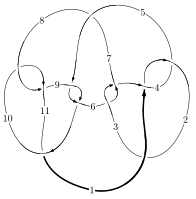
\includegraphics[width=112pt]{../../../GIT/diagram.site/Diagrams/png/263_11a_14.png}\\
\ \ \ A knot diagram\footnotemark}&
\allowdisplaybreaks
\textbf{Linearized knot diagam} \\
\cline{2-2}
 &
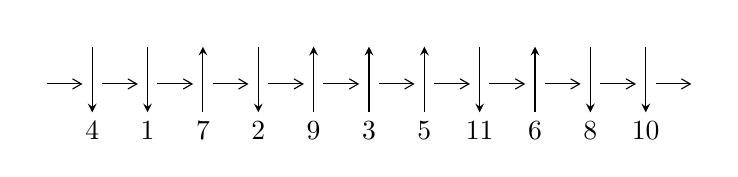
\begin{tikzpicture}[x=20pt, y=17pt]
	% nodes
	\node (C0) at (0, 0) {};
	\node (C1) at (1, 0) {};
	\node (C1U) at (1, +1) {};
	\node (C1D) at (1, -1) {4};

	\node (C2) at (2, 0) {};
	\node (C2U) at (2, +1) {};
	\node (C2D) at (2, -1) {1};

	\node (C3) at (3, 0) {};
	\node (C3U) at (3, +1) {};
	\node (C3D) at (3, -1) {7};

	\node (C4) at (4, 0) {};
	\node (C4U) at (4, +1) {};
	\node (C4D) at (4, -1) {2};

	\node (C5) at (5, 0) {};
	\node (C5U) at (5, +1) {};
	\node (C5D) at (5, -1) {9};

	\node (C6) at (6, 0) {};
	\node (C6U) at (6, +1) {};
	\node (C6D) at (6, -1) {3};

	\node (C7) at (7, 0) {};
	\node (C7U) at (7, +1) {};
	\node (C7D) at (7, -1) {5};

	\node (C8) at (8, 0) {};
	\node (C8U) at (8, +1) {};
	\node (C8D) at (8, -1) {11};

	\node (C9) at (9, 0) {};
	\node (C9U) at (9, +1) {};
	\node (C9D) at (9, -1) {6};

	\node (C10) at (10, 0) {};
	\node (C10U) at (10, +1) {};
	\node (C10D) at (10, -1) {8};

	\node (C11) at (11, 0) {};
	\node (C11U) at (11, +1) {};
	\node (C11D) at (11, -1) {10};
	\node (C12) at (12, 0) {};

	% arrows
	\draw[->,>={angle 60}]
	(C0) edge (C1) (C1) edge (C2) (C2) edge (C3) (C3) edge (C4) (C4) edge (C5) (C5) edge (C6) (C6) edge (C7) (C7) edge (C8) (C8) edge (C9) (C9) edge (C10) (C10) edge (C11) (C11) edge (C12) ;	\draw[->,>=stealth]
	(C1U) edge (C1D) (C2U) edge (C2D) (C3D) edge (C3U) (C4U) edge (C4D) (C5D) edge (C5U) (C6D) edge (C6U) (C7D) edge (C7U) (C8U) edge (C8D) (C9D) edge (C9U) (C10U) edge (C10D) (C11U) edge (C11D) ;
	\end{tikzpicture} \\
\hhline{~~} \\& 
\textbf{Solving Sequence} \\ \cline{2-2} 
 &
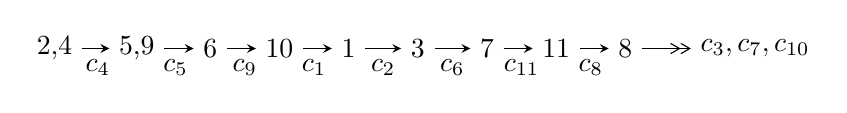
\begin{tikzpicture}[x=25pt, y=7pt]
	% node
	\node (A0) at (-1/8, 0) {2,4};
	\node (A1) at (17/16, 0) {5,9};
	\node (A2) at (17/8, 0) {6};
	\node (A3) at (25/8, 0) {10};
	\node (A4) at (33/8, 0) {1};
	\node (A5) at (41/8, 0) {3};
	\node (A6) at (49/8, 0) {7};
	\node (A7) at (57/8, 0) {11};
	\node (A8) at (65/8, 0) {8};
	\node (C1) at (1/2, -1) {$c_{4}$};
	\node (C2) at (13/8, -1) {$c_{5}$};
	\node (C3) at (21/8, -1) {$c_{9}$};
	\node (C4) at (29/8, -1) {$c_{1}$};
	\node (C5) at (37/8, -1) {$c_{2}$};
	\node (C6) at (45/8, -1) {$c_{6}$};
	\node (C7) at (53/8, -1) {$c_{11}$};
	\node (C8) at (61/8, -1) {$c_{8}$};
	\node (A9) at (10, 0) {$c_{3},c_{7},c_{10}$};

	% edge
	\draw[->,>=stealth]	
	(A0) edge (A1) (A1) edge (A2) (A2) edge (A3) (A3) edge (A4) (A4) edge (A5) (A5) edge (A6) (A6) edge (A7) (A7) edge (A8) ;
	\draw[->>,>={angle 60}]	
	(A8) edge (A9);
\end{tikzpicture} \\ 

\end{tabular} \\

\footnotetext{
The image of knot diagram is generated by the software ``\textbf{Draw programme}" developed by Andrew Bartholomew(\url{http://www.layer8.co.uk/maths/draw/index.htm\#Running-draw}), where we modified some parts for our purpose(\url{https://github.com/CATsTAILs/LinksPainter}).
}\phantom \\ \newline 
\centering \textbf{Ideals for irreducible components\footnotemark of $X_{\text{par}}$} 
 
\begin{align*}
I^u_{1}&=\langle 
u^{11}-2 u^{10}- u^9+5 u^8-2 u^7-5 u^6+5 u^5+2 u^4-5 u^3+u^2+b+u,\\
\phantom{I^u_{1}}&\phantom{= \langle  }u^{11}-2 u^{10}- u^9+5 u^8-2 u^7-5 u^6+5 u^5+u^4-5 u^3+2 u^2+a+u-1,\\
\phantom{I^u_{1}}&\phantom{= \langle  }u^{12}-2 u^{11}- u^{10}+6 u^9-3 u^8-6 u^7+8 u^6+u^5-8 u^4+4 u^3+3 u^2-3 u+1\rangle \\
I^u_{2}&=\langle 
-1.93535\times10^{18} u^{65}-2.98312\times10^{18} u^{64}+\cdots+1.31154\times10^{18} b-9.50336\times10^{18},\\
\phantom{I^u_{2}}&\phantom{= \langle  }1.46340\times10^{19} u^{65}-7.80076\times10^{19} u^{64}+\cdots+6.55768\times10^{17} a-1.85522\times10^{19},\;u^{66}-6 u^{65}+\cdots+u+1\rangle \\
I^u_{3}&=\langle 
- u^5+u^4- u^2+b,\;- u^3+u^2+a-1,\;u^6- u^5- u^4+2 u^3- u+1\rangle \\
I^u_{4}&=\langle 
-2 a^5+2 a^4-7 a^3+5 a^2+3 b-4 a+4,\;a^6+4 a^4+a^3+4 a^2+1,\;u+1\rangle \\
\\
\end{align*}
\raggedright * 4 irreducible components of $\dim_{\mathbb{C}}=0$, with total 90 representations.\\
\footnotetext{All coefficients of polynomials are rational numbers. But the coefficients are sometimes approximated in decimal forms when there is not enough margin.}
\newpage
\renewcommand{\arraystretch}{1}
\centering \section*{I. $I^u_{1}= \langle u^{11}-2 u^{10}+\cdots+b+u,\;u^{11}-2 u^{10}+\cdots+a-1,\;u^{12}-2 u^{11}+\cdots-3 u+1 \rangle$}
\flushleft \textbf{(i) Arc colorings}\\
\begin{tabular}{m{7pt} m{180pt} m{7pt} m{180pt} }
\flushright $a_{2}=$&$\begin{pmatrix}0\\u\end{pmatrix}$ \\
\flushright $a_{4}=$&$\begin{pmatrix}1\\0\end{pmatrix}$ \\
\flushright $a_{5}=$&$\begin{pmatrix}1\\u^2\end{pmatrix}$ \\
\flushright $a_{9}=$&$\begin{pmatrix}- u^{11}+2 u^{10}+u^9-5 u^8+2 u^7+5 u^6-5 u^5- u^4+5 u^3-2 u^2- u+1\\- u^{11}+2 u^{10}+u^9-5 u^8+2 u^7+5 u^6-5 u^5-2 u^4+5 u^3- u^2- u\end{pmatrix}$ \\
\flushright $a_{6}=$&$\begin{pmatrix}- u^9+u^8+2 u^7-3 u^6- u^5+3 u^4- u^3-2 u^2+u+1\\- u^{11}+u^{10}+2 u^9-3 u^8- u^7+3 u^6- u^5-2 u^4+2 u^3+u^2- u\end{pmatrix}$ \\
\flushright $a_{10}=$&$\begin{pmatrix}- u^{11}+2 u^{10}+u^9-5 u^8+2 u^7+4 u^6-5 u^5+4 u^3-2 u^2- u\\- u^{11}+2 u^{10}+u^9-5 u^8+2 u^7+4 u^6-5 u^5+4 u^3-2 u^2\end{pmatrix}$ \\
\flushright $a_{1}=$&$\begin{pmatrix}u\\u\end{pmatrix}$ \\
\flushright $a_{3}=$&$\begin{pmatrix}- u^3\\- u^3+u\end{pmatrix}$ \\
\flushright $a_{7}=$&$\begin{pmatrix}u^{11}- u^{10}-3 u^9+4 u^8+3 u^7-7 u^6+u^5+6 u^4-5 u^3-3 u^2+3 u\\- u^{11}+u^{10}+2 u^9-4 u^8- u^7+5 u^6-2 u^5-4 u^4+3 u^3+u^2-2 u\end{pmatrix}$ \\
\flushright $a_{11}=$&$\begin{pmatrix}- u^{10}+u^9+2 u^8-3 u^7- u^6+4 u^5-2 u^4-2 u^3+3 u^2\\- u^{10}+u^9+2 u^8-3 u^7- u^6+4 u^5-2 u^4-3 u^3+3 u^2\end{pmatrix}$ \\
\flushright $a_{8}=$&$\begin{pmatrix}u^{10}- u^9-2 u^8+3 u^7+u^6-3 u^5+u^4+2 u^3-2 u^2- u+1\\u^{10}- u^9-2 u^8+3 u^7+u^6-3 u^5+u^4+2 u^3- u^2- u\end{pmatrix}$\\ \flushright $a_{8}=$&$\begin{pmatrix}u^{10}- u^9-2 u^8+3 u^7+u^6-3 u^5+u^4+2 u^3-2 u^2- u+1\\u^{10}- u^9-2 u^8+3 u^7+u^6-3 u^5+u^4+2 u^3- u^2- u\end{pmatrix}$\\&\end{tabular}
\flushleft \textbf{(ii) Obstruction class $= -1$}\\~\\
\flushleft \textbf{(iii) Cusp Shapes $= 4 u^{11}-4 u^{10}-4 u^9+8 u^8+4 u^7-8 u^6+4 u^5+12 u^4-4 u^3-4 u^2+4 u+6$}\\~\\
\newpage\renewcommand{\arraystretch}{1}
\flushleft \textbf{(iv) u-Polynomials at the component}\newline \\
\begin{tabular}{m{50pt}|m{274pt}}
Crossings & \hspace{64pt}u-Polynomials at each crossing \\
\hline $$\begin{aligned}c_{1},c_{4},c_{8}\\c_{10}\end{aligned}$$&$\begin{aligned}
&u^{12}-2 u^{11}+\cdots-3 u+1
\end{aligned}$\\
\hline $$\begin{aligned}c_{2},c_{11}\end{aligned}$$&$\begin{aligned}
&u^{12}+6 u^{11}+\cdots+3 u+1
\end{aligned}$\\
\hline $$\begin{aligned}c_{3},c_{5},c_{6}\\c_{9}\end{aligned}$$&$\begin{aligned}
&u^{12}-3 u^{10}+5 u^8+2 u^7-2 u^6-5 u^5+4 u^3+u^2-3 u+1
\end{aligned}$\\
\hline $$\begin{aligned}c_{7}\end{aligned}$$&$\begin{aligned}
&u^{12}+7 u^{11}+\cdots+36 u+8
\end{aligned}$\\
\hline
\end{tabular}\\~\\
\newpage\renewcommand{\arraystretch}{1}
\flushleft \textbf{(v) Riley Polynomials at the component}\newline \\
\begin{tabular}{m{50pt}|m{274pt}}
Crossings & \hspace{64pt}Riley Polynomials at each crossing \\
\hline $$\begin{aligned}c_{1},c_{4},c_{8}\\c_{10}\end{aligned}$$&$\begin{aligned}
&y^{12}-6 y^{11}+\cdots-3 y+1
\end{aligned}$\\
\hline $$\begin{aligned}c_{2},c_{11}\end{aligned}$$&$\begin{aligned}
&y^{12}+2 y^{11}+\cdots+25 y+1
\end{aligned}$\\
\hline $$\begin{aligned}c_{3},c_{5},c_{6}\\c_{9}\end{aligned}$$&$\begin{aligned}
&y^{12}-6 y^{11}+\cdots-7 y+1
\end{aligned}$\\
\hline $$\begin{aligned}c_{7}\end{aligned}$$&$\begin{aligned}
&y^{12}-5 y^{11}+\cdots-112 y+64
\end{aligned}$\\
\hline
\end{tabular}\\~\\
\newpage\flushleft \textbf{(vi) Complex Volumes and Cusp Shapes}
$$\begin{array}{c|c|c}  
\text{Solutions to }I^u_{1}& \I (\text{vol} + \sqrt{-1}CS) & \text{Cusp shape}\\
 \hline 
\begin{aligned}
u &= \phantom{-}0.453738 + 0.929754 I \\
a &= \phantom{-}1.66040 - 0.06848 I \\
b &= \phantom{-}0.28000 + 1.88655 I\end{aligned}
 & \phantom{-}8.07063 + 4.68351 I & \phantom{-}6.05114 - 1.98346 I \\ \hline\begin{aligned}
u &= \phantom{-}0.453738 - 0.929754 I \\
a &= \phantom{-}1.66040 + 0.06848 I \\
b &= \phantom{-}0.28000 - 1.88655 I\end{aligned}
 & \phantom{-}8.07063 - 4.68351 I & \phantom{-}6.05114 + 1.98346 I \\ \hline\begin{aligned}
u &= -0.926778 + 0.513866 I \\
a &= -0.968427 - 0.613844 I \\
b &= -0.820207 - 0.433144 I\end{aligned}
 & -1.88434 + 4.01879 I & -2.34862 - 5.57352 I \\ \hline\begin{aligned}
u &= -0.926778 - 0.513866 I \\
a &= -0.968427 + 0.613844 I \\
b &= -0.820207 + 0.433144 I\end{aligned}
 & -1.88434 - 4.01879 I & -2.34862 + 5.57352 I \\ \hline\begin{aligned}
u &= -1.117600 + 0.115595 I \\
a &= -1.48773 - 1.21599 I \\
b &= -2.71217 - 0.83584 I\end{aligned}
 & -3.84373 + 0.16285 I & \phantom{-}1.32343 + 10.94047 I \\ \hline\begin{aligned}
u &= -1.117600 - 0.115595 I \\
a &= -1.48773 + 1.21599 I \\
b &= -2.71217 + 0.83584 I\end{aligned}
 & -3.84373 - 0.16285 I & \phantom{-}1.32343 - 10.94047 I \\ \hline\begin{aligned}
u &= \phantom{-}1.046970 + 0.439905 I \\
a &= -0.128616 + 1.041170 I \\
b &= -0.192235 + 0.299420 I\end{aligned}
 & -2.42744 - 7.70164 I & -2.21070 + 10.86632 I \\ \hline\begin{aligned}
u &= \phantom{-}1.046970 - 0.439905 I \\
a &= -0.128616 - 1.041170 I \\
b &= -0.192235 - 0.299420 I\end{aligned}
 & -2.42744 + 7.70164 I & -2.21070 - 10.86632 I \\ \hline\begin{aligned}
u &= \phantom{-}1.166620 + 0.659880 I \\
a &= -1.38335 - 1.68558 I \\
b &= \phantom{-}0.05610 - 2.99601 I\end{aligned}
 & \phantom{-}3.6549 - 16.4066 I & \phantom{-}0.26530 + 10.19553 I \\ \hline\begin{aligned}
u &= \phantom{-}1.166620 - 0.659880 I \\
a &= -1.38335 + 1.68558 I \\
b &= \phantom{-}0.05610 + 2.99601 I\end{aligned}
 & \phantom{-}3.6549 + 16.4066 I & \phantom{-}0.26530 - 10.19553 I\\
 \hline 
 \end{array}$$\newpage$$\begin{array}{c|c|c}  
\text{Solutions to }I^u_{1}& \I (\text{vol} + \sqrt{-1}CS) & \text{Cusp shape}\\
 \hline 
\begin{aligned}
u &= \phantom{-}0.377048 + 0.377232 I \\
a &= \phantom{-}0.307725 - 0.384276 I \\
b &= -0.611491 - 0.099728 I\end{aligned}
 & \phantom{-}1.364800 + 0.359490 I & \phantom{-}6.91945 - 0.04590 I \\ \hline\begin{aligned}
u &= \phantom{-}0.377048 - 0.377232 I \\
a &= \phantom{-}0.307725 + 0.384276 I \\
b &= -0.611491 + 0.099728 I\end{aligned}
 & \phantom{-}1.364800 - 0.359490 I & \phantom{-}6.91945 + 0.04590 I\\
 \hline 
 \end{array}$$\newpage\newpage\renewcommand{\arraystretch}{1}
\centering \section*{II. $I^u_{2}= \langle -1.94\times10^{18} u^{65}-2.98\times10^{18} u^{64}+\cdots+1.31\times10^{18} b-9.50\times10^{18},\;1.46\times10^{19} u^{65}-7.80\times10^{19} u^{64}+\cdots+6.56\times10^{17} a-1.86\times10^{19},\;u^{66}-6 u^{65}+\cdots+u+1 \rangle$}
\flushleft \textbf{(i) Arc colorings}\\
\begin{tabular}{m{7pt} m{180pt} m{7pt} m{180pt} }
\flushright $a_{2}=$&$\begin{pmatrix}0\\u\end{pmatrix}$ \\
\flushright $a_{4}=$&$\begin{pmatrix}1\\0\end{pmatrix}$ \\
\flushright $a_{5}=$&$\begin{pmatrix}1\\u^2\end{pmatrix}$ \\
\flushright $a_{9}=$&$\begin{pmatrix}-22.3158 u^{65}+118.956 u^{64}+\cdots+46.5353 u+28.2908\\1.47564 u^{65}+2.27453 u^{64}+\cdots+16.1199 u+7.24598\end{pmatrix}$ \\
\flushright $a_{6}=$&$\begin{pmatrix}17.6460 u^{65}-85.9310 u^{64}+\cdots-5.54679 u-12.6993\\-9.07917 u^{65}+44.9975 u^{64}+\cdots+7.67709 u+6.14426\end{pmatrix}$ \\
\flushright $a_{10}=$&$\begin{pmatrix}-19.4674 u^{65}+106.132 u^{64}+\cdots+53.5854 u+28.9858\\-6.78423 u^{65}+40.7932 u^{64}+\cdots+19.6572 u+11.6136\end{pmatrix}$ \\
\flushright $a_{1}=$&$\begin{pmatrix}u\\u\end{pmatrix}$ \\
\flushright $a_{3}=$&$\begin{pmatrix}- u^3\\- u^3+u\end{pmatrix}$ \\
\flushright $a_{7}=$&$\begin{pmatrix}35.5665 u^{65}-177.684 u^{64}+\cdots-30.3716 u-28.2580\\-0.424705 u^{65}-6.71788 u^{64}+\cdots-25.7126 u-8.98968\end{pmatrix}$ \\
\flushright $a_{11}=$&$\begin{pmatrix}25.6164 u^{65}-133.621 u^{64}+\cdots-36.9797 u-29.4827\\-8.13884 u^{65}+30.6283 u^{64}+\cdots-9.28517 u-2.65549\end{pmatrix}$ \\
\flushright $a_{8}=$&$\begin{pmatrix}6.14426 u^{65}-27.7864 u^{64}+\cdots+15.1971 u-1.53283\\-19.9447 u^{65}+100.602 u^{64}+\cdots+30.3453 u+17.6460\end{pmatrix}$\\ \flushright $a_{8}=$&$\begin{pmatrix}6.14426 u^{65}-27.7864 u^{64}+\cdots+15.1971 u-1.53283\\-19.9447 u^{65}+100.602 u^{64}+\cdots+30.3453 u+17.6460\end{pmatrix}$\\&\end{tabular}
\flushleft \textbf{(ii) Obstruction class $= -1$}\\~\\
\flushleft \textbf{(iii) Cusp Shapes $= \frac{12086631496832904775}{655767731184955984} u^{65}-\frac{7581252097116615619}{81970966398119498} u^{64}+\cdots-\frac{441245495247013113}{655767731184955984} u-\frac{4211855983240591645}{327883865592477992}$}\\~\\
\newpage\renewcommand{\arraystretch}{1}
\flushleft \textbf{(iv) u-Polynomials at the component}\newline \\
\begin{tabular}{m{50pt}|m{274pt}}
Crossings & \hspace{64pt}u-Polynomials at each crossing \\
\hline $$\begin{aligned}c_{1},c_{4},c_{8}\\c_{10}\end{aligned}$$&$\begin{aligned}
&u^{66}-6 u^{65}+\cdots+u+1
\end{aligned}$\\
\hline $$\begin{aligned}c_{2},c_{11}\end{aligned}$$&$\begin{aligned}
&u^{66}+30 u^{65}+\cdots-25 u+1
\end{aligned}$\\
\hline $$\begin{aligned}c_{3},c_{5},c_{6}\\c_{9}\end{aligned}$$&$\begin{aligned}
&u^{66}-2 u^{65}+\cdots-64 u+64
\end{aligned}$\\
\hline $$\begin{aligned}c_{7}\end{aligned}$$&$\begin{aligned}
&(u^{33}-2 u^{32}+\cdots+84 u+49)^{2}
\end{aligned}$\\
\hline
\end{tabular}\\~\\
\newpage\renewcommand{\arraystretch}{1}
\flushleft \textbf{(v) Riley Polynomials at the component}\newline \\
\begin{tabular}{m{50pt}|m{274pt}}
Crossings & \hspace{64pt}Riley Polynomials at each crossing \\
\hline $$\begin{aligned}c_{1},c_{4},c_{8}\\c_{10}\end{aligned}$$&$\begin{aligned}
&y^{66}-30 y^{65}+\cdots+25 y+1
\end{aligned}$\\
\hline $$\begin{aligned}c_{2},c_{11}\end{aligned}$$&$\begin{aligned}
&y^{66}+18 y^{65}+\cdots+1453 y+1
\end{aligned}$\\
\hline $$\begin{aligned}c_{3},c_{5},c_{6}\\c_{9}\end{aligned}$$&$\begin{aligned}
&y^{66}-36 y^{65}+\cdots-36864 y+4096
\end{aligned}$\\
\hline $$\begin{aligned}c_{7}\end{aligned}$$&$\begin{aligned}
&(y^{33}-14 y^{32}+\cdots-3528 y-2401)^{2}
\end{aligned}$\\
\hline
\end{tabular}\\~\\
\newpage\flushleft \textbf{(vi) Complex Volumes and Cusp Shapes}
$$\begin{array}{c|c|c}  
\text{Solutions to }I^u_{2}& \I (\text{vol} + \sqrt{-1}CS) & \text{Cusp shape}\\
 \hline 
\begin{aligned}
u &= -0.904759 + 0.446690 I \\
a &= \phantom{-}2.84122 - 1.52553 I \\
b &= \phantom{-}1.32232 - 3.04286 I\end{aligned}
 & -2.95867 + 1.76219 I & \phantom{-0.000000 } 0 \\ \hline\begin{aligned}
u &= -0.904759 - 0.446690 I \\
a &= \phantom{-}2.84122 + 1.52553 I \\
b &= \phantom{-}1.32232 + 3.04286 I\end{aligned}
 & -2.95867 - 1.76219 I & \phantom{-0.000000 } 0 \\ \hline\begin{aligned}
u &= \phantom{-}0.544139 + 0.827076 I \\
a &= \phantom{-}0.172505 - 0.275088 I \\
b &= \phantom{-}0.107638 - 0.791057 I\end{aligned}
 & \phantom{-}3.57176 - 0.40211 I & \phantom{-0.000000 } 0 \\ \hline\begin{aligned}
u &= \phantom{-}0.544139 - 0.827076 I \\
a &= \phantom{-}0.172505 + 0.275088 I \\
b &= \phantom{-}0.107638 + 0.791057 I\end{aligned}
 & \phantom{-}3.57176 + 0.40211 I & \phantom{-0.000000 } 0 \\ \hline\begin{aligned}
u &= -0.961832 + 0.210042 I \\
a &= \phantom{-}0.756823 - 0.566102 I \\
b &= \phantom{-}0.636013 - 0.444310 I\end{aligned}
 & -1.74022 + 0.71657 I & \phantom{-0.000000 } 0 \\ \hline\begin{aligned}
u &= -0.961832 - 0.210042 I \\
a &= \phantom{-}0.756823 + 0.566102 I \\
b &= \phantom{-}0.636013 + 0.444310 I\end{aligned}
 & -1.74022 - 0.71657 I & \phantom{-0.000000 } 0 \\ \hline\begin{aligned}
u &= \phantom{-}0.455132 + 0.872435 I \\
a &= -0.321275 + 0.229842 I \\
b &= -0.339251 + 0.707485 I\end{aligned}
 & \phantom{-}2.96228 + 4.26802 I & \phantom{-0.000000 } 0 \\ \hline\begin{aligned}
u &= \phantom{-}0.455132 - 0.872435 I \\
a &= -0.321275 - 0.229842 I \\
b &= -0.339251 - 0.707485 I\end{aligned}
 & \phantom{-}2.96228 - 4.26802 I & \phantom{-0.000000 } 0 \\ \hline\begin{aligned}
u &= \phantom{-}0.407462 + 0.942447 I \\
a &= -1.49558 + 0.17696 I \\
b &= -0.33336 - 1.92881 I\end{aligned}
 & \phantom{-}5.96795 + 10.55640 I & \phantom{-0.000000 } 0 \\ \hline\begin{aligned}
u &= \phantom{-}0.407462 - 0.942447 I \\
a &= -1.49558 - 0.17696 I \\
b &= -0.33336 + 1.92881 I\end{aligned}
 & \phantom{-}5.96795 - 10.55640 I & \phantom{-0.000000 } 0\\
 \hline 
 \end{array}$$\newpage$$\begin{array}{c|c|c}  
\text{Solutions to }I^u_{2}& \I (\text{vol} + \sqrt{-1}CS) & \text{Cusp shape}\\
 \hline 
\begin{aligned}
u &= \phantom{-}0.914238 + 0.471505 I \\
a &= \phantom{-}0.274153 - 0.838704 I \\
b &= \phantom{-}1.65746 + 0.36585 I\end{aligned}
 & -2.80746 - 3.11554 I & \phantom{-0.000000 } 0 \\ \hline\begin{aligned}
u &= \phantom{-}0.914238 - 0.471505 I \\
a &= \phantom{-}0.274153 + 0.838704 I \\
b &= \phantom{-}1.65746 - 0.36585 I\end{aligned}
 & -2.80746 + 3.11554 I & \phantom{-0.000000 } 0 \\ \hline\begin{aligned}
u &= \phantom{-}0.862360 + 0.437489 I \\
a &= \phantom{-}0.51258 + 1.50106 I \\
b &= -0.216752 + 0.388716 I\end{aligned}
 & -2.55962 - 0.56819 I & \phantom{-0.000000 } 0 \\ \hline\begin{aligned}
u &= \phantom{-}0.862360 - 0.437489 I \\
a &= \phantom{-}0.51258 - 1.50106 I \\
b &= -0.216752 - 0.388716 I\end{aligned}
 & -2.55962 + 0.56819 I & \phantom{-0.000000 } 0 \\ \hline\begin{aligned}
u &= \phantom{-}0.480350 + 0.829100 I \\
a &= -2.22215 + 0.10328 I \\
b &= -0.03293 - 1.98412 I\end{aligned}
 & \phantom{-}1.71328 + 1.77212 I & \phantom{-0.000000 } 0 \\ \hline\begin{aligned}
u &= \phantom{-}0.480350 - 0.829100 I \\
a &= -2.22215 - 0.10328 I \\
b &= -0.03293 + 1.98412 I\end{aligned}
 & \phantom{-}1.71328 - 1.77212 I & \phantom{-0.000000 } 0 \\ \hline\begin{aligned}
u &= -0.732260 + 0.589717 I \\
a &= -2.12270 + 0.89719 I \\
b &= -0.87763 + 2.26509 I\end{aligned}
 & \phantom{-}3.57176 + 0.40211 I & \phantom{-}3.54240 + 0. I\phantom{ +0.000000I} \\ \hline\begin{aligned}
u &= -0.732260 - 0.589717 I \\
a &= -2.12270 - 0.89719 I \\
b &= -0.87763 - 2.26509 I\end{aligned}
 & \phantom{-}3.57176 - 0.40211 I & \phantom{-}3.54240 + 0. I\phantom{ +0.000000I} \\ \hline\begin{aligned}
u &= \phantom{-}0.603634 + 0.892529 I \\
a &= \phantom{-}1.83672 + 0.40288 I \\
b &= \phantom{-}0.14265 + 1.57592 I\end{aligned}
 & \phantom{-}9.06216\phantom{ +0.000000I} & \phantom{-0.000000 } 0 \\ \hline\begin{aligned}
u &= \phantom{-}0.603634 - 0.892529 I \\
a &= \phantom{-}1.83672 - 0.40288 I \\
b &= \phantom{-}0.14265 - 1.57592 I\end{aligned}
 & \phantom{-}9.06216\phantom{ +0.000000I} & \phantom{-0.000000 } 0\\
 \hline 
 \end{array}$$\newpage$$\begin{array}{c|c|c}  
\text{Solutions to }I^u_{2}& \I (\text{vol} + \sqrt{-1}CS) & \text{Cusp shape}\\
 \hline 
\begin{aligned}
u &= -0.929321 + 0.583508 I \\
a &= -2.15255 + 1.50339 I \\
b &= -0.74412 + 2.72281 I\end{aligned}
 & \phantom{-}2.96228 + 4.26802 I & \phantom{-0.000000 } 0 \\ \hline\begin{aligned}
u &= -0.929321 - 0.583508 I \\
a &= -2.15255 - 1.50339 I \\
b &= -0.74412 - 2.72281 I\end{aligned}
 & \phantom{-}2.96228 - 4.26802 I & \phantom{-0.000000 } 0 \\ \hline\begin{aligned}
u &= \phantom{-}0.665888 + 0.873727 I \\
a &= -1.77794 - 0.54323 I \\
b &= -0.133969 - 1.404830 I\end{aligned}
 & \phantom{-}7.69426 - 5.94756 I & \phantom{-0.000000 } 0 \\ \hline\begin{aligned}
u &= \phantom{-}0.665888 - 0.873727 I \\
a &= -1.77794 + 0.54323 I \\
b &= -0.133969 + 1.404830 I\end{aligned}
 & \phantom{-}7.69426 + 5.94756 I & \phantom{-0.000000 } 0 \\ \hline\begin{aligned}
u &= \phantom{-}0.957231 + 0.541430 I \\
a &= -0.526732 - 0.892898 I \\
b &= \phantom{-}0.065036 - 0.385894 I\end{aligned}
 & \phantom{-}0.32108 - 4.39805 I & \phantom{-0.000000 } 0 \\ \hline\begin{aligned}
u &= \phantom{-}0.957231 - 0.541430 I \\
a &= -0.526732 + 0.892898 I \\
b &= \phantom{-}0.065036 + 0.385894 I\end{aligned}
 & \phantom{-}0.32108 + 4.39805 I & \phantom{-0.000000 } 0 \\ \hline\begin{aligned}
u &= \phantom{-}0.853729 + 0.285494 I \\
a &= -0.543347 - 0.659944 I \\
b &= \phantom{-}1.020820 - 0.059850 I\end{aligned}
 & -1.19449 + 4.90633 I & \phantom{-}1.49511 + 0. I\phantom{ +0.000000I} \\ \hline\begin{aligned}
u &= \phantom{-}0.853729 - 0.285494 I \\
a &= -0.543347 + 0.659944 I \\
b &= \phantom{-}1.020820 + 0.059850 I\end{aligned}
 & -1.19449 - 4.90633 I & \phantom{-}1.49511 + 0. I\phantom{ +0.000000I} \\ \hline\begin{aligned}
u &= -0.770621 + 0.443457 I \\
a &= \phantom{-}1.182830 + 0.436102 I \\
b &= \phantom{-}0.913903 + 0.253008 I\end{aligned}
 & -1.31058\phantom{ +0.000000I} &                 -6
-1.00000 + 0. 10   I\phantom{ +0.000000I} \\ \hline\begin{aligned}
u &= -0.770621 - 0.443457 I \\
a &= \phantom{-}1.182830 - 0.436102 I \\
b &= \phantom{-}0.913903 - 0.253008 I\end{aligned}
 & -1.31058\phantom{ +0.000000I} &                 -6
-1.00000 + 0. 10   I\phantom{ +0.000000I}\\
 \hline 
 \end{array}$$\newpage$$\begin{array}{c|c|c}  
\text{Solutions to }I^u_{2}& \I (\text{vol} + \sqrt{-1}CS) & \text{Cusp shape}\\
 \hline 
\begin{aligned}
u &= -0.636940 + 0.614253 I \\
a &= \phantom{-}1.97230 - 0.67580 I \\
b &= \phantom{-}0.75955 - 2.09262 I\end{aligned}
 & \phantom{-}1.98821 - 5.14475 I & \phantom{-}1.15894 + 2.87802 I \\ \hline\begin{aligned}
u &= -0.636940 - 0.614253 I \\
a &= \phantom{-}1.97230 + 0.67580 I \\
b &= \phantom{-}0.75955 + 2.09262 I\end{aligned}
 & \phantom{-}1.98821 + 5.14475 I & \phantom{-}1.15894 - 2.87802 I \\ \hline\begin{aligned}
u &= -0.982708 + 0.588767 I \\
a &= \phantom{-}2.05598 - 1.64453 I \\
b &= \phantom{-}0.60719 - 2.77532 I\end{aligned}
 & \phantom{-}0.94779 + 9.91324 I & \phantom{-0.000000 } 0 \\ \hline\begin{aligned}
u &= -0.982708 - 0.588767 I \\
a &= \phantom{-}2.05598 + 1.64453 I \\
b &= \phantom{-}0.60719 + 2.77532 I\end{aligned}
 & \phantom{-}0.94779 - 9.91324 I & \phantom{-0.000000 } 0 \\ \hline\begin{aligned}
u &= \phantom{-}0.726072 + 0.397331 I \\
a &= \phantom{-}0.228530 + 0.275068 I \\
b &= -0.921432 - 0.266276 I\end{aligned}
 & \phantom{-}1.240670 + 0.272253 I & \phantom{-}4.90559 + 1.40386 I \\ \hline\begin{aligned}
u &= \phantom{-}0.726072 - 0.397331 I \\
a &= \phantom{-}0.228530 - 0.275068 I \\
b &= -0.921432 + 0.266276 I\end{aligned}
 & \phantom{-}1.240670 - 0.272253 I & \phantom{-}4.90559 - 1.40386 I \\ \hline\begin{aligned}
u &= -1.115560 + 0.407709 I \\
a &= -0.525366 - 0.866763 I \\
b &= -0.470438 - 0.713792 I\end{aligned}
 & -2.55962 - 0.56819 I & \phantom{-0.000000 } 0 \\ \hline\begin{aligned}
u &= -1.115560 - 0.407709 I \\
a &= -0.525366 + 0.866763 I \\
b &= -0.470438 + 0.713792 I\end{aligned}
 & -2.55962 + 0.56819 I & \phantom{-0.000000 } 0 \\ \hline\begin{aligned}
u &= -1.228300 + 0.089688 I \\
a &= \phantom{-}0.00030 + 1.42724 I \\
b &= \phantom{-}0.001942 + 1.245290 I\end{aligned}
 & -2.95867 - 1.76219 I & \phantom{-0.000000 } 0 \\ \hline\begin{aligned}
u &= -1.228300 - 0.089688 I \\
a &= \phantom{-}0.00030 - 1.42724 I \\
b &= \phantom{-}0.001942 - 1.245290 I\end{aligned}
 & -2.95867 + 1.76219 I & \phantom{-0.000000 } 0\\
 \hline 
 \end{array}$$\newpage$$\begin{array}{c|c|c}  
\text{Solutions to }I^u_{2}& \I (\text{vol} + \sqrt{-1}CS) & \text{Cusp shape}\\
 \hline 
\begin{aligned}
u &= -1.195920 + 0.308871 I \\
a &= \phantom{-}0.280220 + 1.105220 I \\
b &= \phantom{-}0.260029 + 0.942647 I\end{aligned}
 & -2.80746 + 3.11554 I & \phantom{-0.000000 } 0 \\ \hline\begin{aligned}
u &= -1.195920 - 0.308871 I \\
a &= \phantom{-}0.280220 - 1.105220 I \\
b &= \phantom{-}0.260029 - 0.942647 I\end{aligned}
 & -2.80746 - 3.11554 I & \phantom{-0.000000 } 0 \\ \hline\begin{aligned}
u &= \phantom{-}1.117620 + 0.541451 I \\
a &= \phantom{-}0.455569 - 0.426873 I \\
b &= \phantom{-}0.251455 - 0.081822 I\end{aligned}
 & -1.19449 - 4.90633 I & \phantom{-0.000000 } 0 \\ \hline\begin{aligned}
u &= \phantom{-}1.117620 - 0.541451 I \\
a &= \phantom{-}0.455569 + 0.426873 I \\
b &= \phantom{-}0.251455 + 0.081822 I\end{aligned}
 & -1.19449 + 4.90633 I & \phantom{-0.000000 } 0 \\ \hline\begin{aligned}
u &= \phantom{-}1.002330 + 0.741441 I \\
a &= -0.967924 - 0.751179 I \\
b &= -0.66959 - 2.18374 I\end{aligned}
 & \phantom{-}6.67035\phantom{ +0.000000I} & \phantom{-0.000000 } 0 \\ \hline\begin{aligned}
u &= \phantom{-}1.002330 - 0.741441 I \\
a &= -0.967924 + 0.751179 I \\
b &= -0.66959 + 2.18374 I\end{aligned}
 & \phantom{-}6.67035\phantom{ +0.000000I} & \phantom{-0.000000 } 0 \\ \hline\begin{aligned}
u &= \phantom{-}1.067510 + 0.658022 I \\
a &= -0.869685 - 0.189017 I \\
b &= -0.302076 - 0.305752 I\end{aligned}
 & \phantom{-}1.98821 - 5.14475 I & \phantom{-0.000000 } 0 \\ \hline\begin{aligned}
u &= \phantom{-}1.067510 - 0.658022 I \\
a &= -0.869685 + 0.189017 I \\
b &= -0.302076 + 0.305752 I\end{aligned}
 & \phantom{-}1.98821 + 5.14475 I & \phantom{-0.000000 } 0 \\ \hline\begin{aligned}
u &= \phantom{-}1.100320 + 0.643486 I \\
a &= -1.82351 - 1.35338 I \\
b &= -0.53477 - 3.38382 I\end{aligned}
 & -0.15117 - 7.27375 I & \phantom{-0.000000 } 0 \\ \hline\begin{aligned}
u &= \phantom{-}1.100320 - 0.643486 I \\
a &= -1.82351 + 1.35338 I \\
b &= -0.53477 + 3.38382 I\end{aligned}
 & -0.15117 + 7.27375 I & \phantom{-0.000000 } 0\\
 \hline 
 \end{array}$$\newpage$$\begin{array}{c|c|c}  
\text{Solutions to }I^u_{2}& \I (\text{vol} + \sqrt{-1}CS) & \text{Cusp shape}\\
 \hline 
\begin{aligned}
u &= \phantom{-}1.053810 + 0.724277 I \\
a &= \phantom{-}1.17869 + 0.95847 I \\
b &= \phantom{-}0.61114 + 2.49765 I\end{aligned}
 & \phantom{-}7.69426 - 5.94756 I & \phantom{-0.000000 } 0 \\ \hline\begin{aligned}
u &= \phantom{-}1.053810 - 0.724277 I \\
a &= \phantom{-}1.17869 - 0.95847 I \\
b &= \phantom{-}0.61114 - 2.49765 I\end{aligned}
 & \phantom{-}7.69426 + 5.94756 I & \phantom{-0.000000 } 0 \\ \hline\begin{aligned}
u &= \phantom{-}1.122900 + 0.653215 I \\
a &= \phantom{-}0.911720 - 0.036398 I \\
b &= \phantom{-}0.401683 + 0.200042 I\end{aligned}
 & \phantom{-}0.94779 - 9.91324 I & \phantom{-0.000000 } 0 \\ \hline\begin{aligned}
u &= \phantom{-}1.122900 - 0.653215 I \\
a &= \phantom{-}0.911720 + 0.036398 I \\
b &= \phantom{-}0.401683 - 0.200042 I\end{aligned}
 & \phantom{-}0.94779 + 9.91324 I & \phantom{-0.000000 } 0 \\ \hline\begin{aligned}
u &= -1.307610 + 0.078191 I \\
a &= \phantom{-}0.047475 + 0.477579 I \\
b &= \phantom{-}1.39323 + 0.46432 I\end{aligned}
 & \phantom{-}1.71328 - 1.77212 I & \phantom{-0.000000 } 0 \\ \hline\begin{aligned}
u &= -1.307610 - 0.078191 I \\
a &= \phantom{-}0.047475 - 0.477579 I \\
b &= \phantom{-}1.39323 - 0.46432 I\end{aligned}
 & \phantom{-}1.71328 + 1.77212 I & \phantom{-0.000000 } 0 \\ \hline\begin{aligned}
u &= \phantom{-}0.209151 + 0.653417 I \\
a &= -0.350286 - 0.352621 I \\
b &= -0.604455 + 0.140178 I\end{aligned}
 & \phantom{-}1.240670 + 0.272253 I & \phantom{-}4.90559 + 1.40386 I \\ \hline\begin{aligned}
u &= \phantom{-}0.209151 - 0.653417 I \\
a &= -0.350286 + 0.352621 I \\
b &= -0.604455 - 0.140178 I\end{aligned}
 & \phantom{-}1.240670 - 0.272253 I & \phantom{-}4.90559 - 1.40386 I \\ \hline\begin{aligned}
u &= \phantom{-}1.144110 + 0.674165 I \\
a &= \phantom{-}1.41189 + 1.53805 I \\
b &= \phantom{-}0.13026 + 2.98702 I\end{aligned}
 & \phantom{-}5.96795 - 10.55640 I & \phantom{-0.000000 } 0 \\ \hline\begin{aligned}
u &= \phantom{-}1.144110 - 0.674165 I \\
a &= \phantom{-}1.41189 - 1.53805 I \\
b &= \phantom{-}0.13026 - 2.98702 I\end{aligned}
 & \phantom{-}5.96795 + 10.55640 I & \phantom{-0.000000 } 0\\
 \hline 
 \end{array}$$\newpage$$\begin{array}{c|c|c}  
\text{Solutions to }I^u_{2}& \I (\text{vol} + \sqrt{-1}CS) & \text{Cusp shape}\\
 \hline 
\begin{aligned}
u &= -1.322010 + 0.130704 I \\
a &= \phantom{-}0.130195 - 0.748866 I \\
b &= -1.24973 - 0.75426 I\end{aligned}
 & -0.15117 - 7.27375 I & \phantom{-0.000000 } 0 \\ \hline\begin{aligned}
u &= -1.322010 - 0.130704 I \\
a &= \phantom{-}0.130195 + 0.748866 I \\
b &= -1.24973 + 0.75426 I\end{aligned}
 & -0.15117 + 7.27375 I & \phantom{-0.000000 } 0 \\ \hline\begin{aligned}
u &= -0.114209 + 0.585210 I \\
a &= \phantom{-}0.862900 + 0.756442 I \\
b &= \phantom{-}0.850025 + 0.016896 I\end{aligned}
 & \phantom{-}0.32108 + 4.39805 I & \phantom{-}1.68085 - 6.72354 I \\ \hline\begin{aligned}
u &= -0.114209 - 0.585210 I \\
a &= \phantom{-}0.862900 - 0.756442 I \\
b &= \phantom{-}0.850025 - 0.016896 I\end{aligned}
 & \phantom{-}0.32108 - 4.39805 I & \phantom{-}1.68085 + 6.72354 I \\ \hline\begin{aligned}
u &= -0.085935 + 0.142884 I \\
a &= \phantom{-}4.58644 + 1.21264 I \\
b &= \phantom{-}0.298158 - 0.682511 I\end{aligned}
 & -1.74022 + 0.71657 I & -3.97070 - 0.74474 I \\ \hline\begin{aligned}
u &= -0.085935 - 0.142884 I \\
a &= \phantom{-}4.58644 - 1.21264 I \\
b &= \phantom{-}0.298158 + 0.682511 I\end{aligned}
 & -1.74022 - 0.71657 I & -3.97070 + 0.74474 I\\
 \hline 
 \end{array}$$\newpage\newpage\renewcommand{\arraystretch}{1}
\centering \section*{III. $I^u_{3}= \langle - u^5+u^4- u^2+b,\;- u^3+u^2+a-1,\;u^6- u^5- u^4+2 u^3- u+1 \rangle$}
\flushleft \textbf{(i) Arc colorings}\\
\begin{tabular}{m{7pt} m{180pt} m{7pt} m{180pt} }
\flushright $a_{2}=$&$\begin{pmatrix}0\\u\end{pmatrix}$ \\
\flushright $a_{4}=$&$\begin{pmatrix}1\\0\end{pmatrix}$ \\
\flushright $a_{5}=$&$\begin{pmatrix}1\\u^2\end{pmatrix}$ \\
\flushright $a_{9}=$&$\begin{pmatrix}u^3- u^2+1\\u^5- u^4+u^2\end{pmatrix}$ \\
\flushright $a_{6}=$&$\begin{pmatrix}1\\u^2\end{pmatrix}$ \\
\flushright $a_{10}=$&$\begin{pmatrix}u^3- u^2+1\\u^5- u^4+u^2\end{pmatrix}$ \\
\flushright $a_{1}=$&$\begin{pmatrix}u\\u\end{pmatrix}$ \\
\flushright $a_{3}=$&$\begin{pmatrix}- u^3\\- u^3+u\end{pmatrix}$ \\
\flushright $a_{7}=$&$\begin{pmatrix}- u^3\\- u^5+u^3- u\end{pmatrix}$ \\
\flushright $a_{11}=$&$\begin{pmatrix}u^3- u^2+u+1\\u^5- u^4+u^2+u\end{pmatrix}$ \\
\flushright $a_{8}=$&$\begin{pmatrix}- u\\- u\end{pmatrix}$\\ \flushright $a_{8}=$&$\begin{pmatrix}- u\\- u\end{pmatrix}$\\&\end{tabular}
\flushleft \textbf{(ii) Obstruction class $= 1$}\\~\\
\flushleft \textbf{(iii) Cusp Shapes $= 3 u^4+2 u^3-3 u^2+2 u-1$}\\~\\
\newpage\renewcommand{\arraystretch}{1}
\flushleft \textbf{(iv) u-Polynomials at the component}\newline \\
\begin{tabular}{m{50pt}|m{274pt}}
Crossings & \hspace{64pt}u-Polynomials at each crossing \\
\hline $$\begin{aligned}c_{1},c_{6}\end{aligned}$$&$\begin{aligned}
&u^6+u^5- u^4-2 u^3+u+1
\end{aligned}$\\
\hline $$\begin{aligned}c_{2}\end{aligned}$$&$\begin{aligned}
&u^6+3 u^5+5 u^4+4 u^3+2 u^2+u+1
\end{aligned}$\\
\hline $$\begin{aligned}c_{3},c_{4}\end{aligned}$$&$\begin{aligned}
&u^6- u^5- u^4+2 u^3- u+1
\end{aligned}$\\
\hline $$\begin{aligned}c_{5},c_{9}\end{aligned}$$&$\begin{aligned}
&u^6
\end{aligned}$\\
\hline $$\begin{aligned}c_{7}\end{aligned}$$&$\begin{aligned}
&u^6-3 u^5+5 u^4-4 u^3+2 u^2- u+1
\end{aligned}$\\
\hline $$\begin{aligned}c_{8}\end{aligned}$$&$\begin{aligned}
&(u-1)^6
\end{aligned}$\\
\hline $$\begin{aligned}c_{10},c_{11}\end{aligned}$$&$\begin{aligned}
&(u+1)^6
\end{aligned}$\\
\hline
\end{tabular}\\~\\
\newpage\renewcommand{\arraystretch}{1}
\flushleft \textbf{(v) Riley Polynomials at the component}\newline \\
\begin{tabular}{m{50pt}|m{274pt}}
Crossings & \hspace{64pt}Riley Polynomials at each crossing \\
\hline $$\begin{aligned}c_{1},c_{3},c_{4}\\c_{6}\end{aligned}$$&$\begin{aligned}
&y^6-3 y^5+5 y^4-4 y^3+2 y^2- y+1
\end{aligned}$\\
\hline $$\begin{aligned}c_{2},c_{7}\end{aligned}$$&$\begin{aligned}
&y^6+y^5+5 y^4+6 y^2+3 y+1
\end{aligned}$\\
\hline $$\begin{aligned}c_{5},c_{9}\end{aligned}$$&$\begin{aligned}
&y^6
\end{aligned}$\\
\hline $$\begin{aligned}c_{8},c_{10},c_{11}\end{aligned}$$&$\begin{aligned}
&(y-1)^6
\end{aligned}$\\
\hline
\end{tabular}\\~\\
\newpage\flushleft \textbf{(vi) Complex Volumes and Cusp Shapes}
$$\begin{array}{c|c|c}  
\text{Solutions to }I^u_{3}& \I (\text{vol} + \sqrt{-1}CS) & \text{Cusp shape}\\
 \hline 
\begin{aligned}
u &= -1.002190 + 0.295542 I \\
a &= -0.66103 + 1.45708 I \\
b &= \phantom{-}0.25695 + 1.72779 I\end{aligned}
 & -3.53554 + 0.92430 I & -5.77331 + 0.83820 I \\ \hline\begin{aligned}
u &= -1.002190 - 0.295542 I \\
a &= -0.66103 - 1.45708 I \\
b &= \phantom{-}0.25695 - 1.72779 I\end{aligned}
 & -3.53554 - 0.92430 I & -5.77331 - 0.83820 I \\ \hline\begin{aligned}
u &= \phantom{-}0.428243 + 0.664531 I \\
a &= \phantom{-}0.769407 - 0.497010 I \\
b &= \phantom{-}0.084211 + 0.566250 I\end{aligned}
 & \phantom{-}0.245672 + 0.924305 I & -1.11831 - 1.11590 I \\ \hline\begin{aligned}
u &= \phantom{-}0.428243 - 0.664531 I \\
a &= \phantom{-}0.769407 + 0.497010 I \\
b &= \phantom{-}0.084211 - 0.566250 I\end{aligned}
 & \phantom{-}0.245672 - 0.924305 I & -1.11831 + 1.11590 I \\ \hline\begin{aligned}
u &= \phantom{-}1.073950 + 0.558752 I \\
a &= \phantom{-}0.391622 + 0.558752 I \\
b &= -0.341164 + 0.940004 I\end{aligned}
 & -1.64493 - 5.69302 I & -3.10838 + 7.09196 I \\ \hline\begin{aligned}
u &= \phantom{-}1.073950 - 0.558752 I \\
a &= \phantom{-}0.391622 - 0.558752 I \\
b &= -0.341164 - 0.940004 I\end{aligned}
 & -1.64493 + 5.69302 I & -3.10838 - 7.09196 I\\
 \hline 
 \end{array}$$\newpage\newpage\renewcommand{\arraystretch}{1}
\centering \section*{IV. $I^u_{4}= \langle -2 a^5+2 a^4-7 a^3+5 a^2+3 b-4 a+4,\;a^6+4 a^4+a^3+4 a^2+1,\;u+1 \rangle$}
\flushleft \textbf{(i) Arc colorings}\\
\begin{tabular}{m{7pt} m{180pt} m{7pt} m{180pt} }
\flushright $a_{2}=$&$\begin{pmatrix}0\\-1\end{pmatrix}$ \\
\flushright $a_{4}=$&$\begin{pmatrix}1\\0\end{pmatrix}$ \\
\flushright $a_{5}=$&$\begin{pmatrix}1\\1\end{pmatrix}$ \\
\flushright $a_{9}=$&$\begin{pmatrix}a\\\frac{2}{3} a^5-\frac{2}{3} a^4+\cdots+\frac{4}{3} a-\frac{4}{3}\end{pmatrix}$ \\
\flushright $a_{6}=$&$\begin{pmatrix}\frac{2}{3} a^5+\frac{1}{3} a^4+\cdots+\frac{4}{3} a+\frac{5}{3}\\0\end{pmatrix}$ \\
\flushright $a_{10}=$&$\begin{pmatrix}\frac{1}{3} a^5-\frac{1}{3} a^4+\cdots-\frac{1}{3} a-\frac{2}{3}\\\frac{2}{3} a^5-\frac{2}{3} a^4+\cdots+\frac{4}{3} a-\frac{4}{3}\end{pmatrix}$ \\
\flushright $a_{1}=$&$\begin{pmatrix}-1\\-1\end{pmatrix}$ \\
\flushright $a_{3}=$&$\begin{pmatrix}1\\0\end{pmatrix}$ \\
\flushright $a_{7}=$&$\begin{pmatrix}\frac{2}{3} a^5+\frac{1}{3} a^4+\cdots+\frac{4}{3} a+\frac{5}{3}\\0\end{pmatrix}$ \\
\flushright $a_{11}=$&$\begin{pmatrix}\frac{1}{3} a^5-\frac{1}{3} a^4+\cdots-\frac{1}{3} a-\frac{2}{3}\\-\frac{2}{3} a^5-\frac{1}{3} a^4+\cdots-\frac{4}{3} a-\frac{5}{3}\end{pmatrix}$ \\
\flushright $a_{8}=$&$\begin{pmatrix}0\\-\frac{2}{3} a^5-\frac{1}{3} a^4+\cdots-\frac{4}{3} a-\frac{5}{3}\end{pmatrix}$\\ \flushright $a_{8}=$&$\begin{pmatrix}0\\-\frac{2}{3} a^5-\frac{1}{3} a^4+\cdots-\frac{4}{3} a-\frac{5}{3}\end{pmatrix}$\\&\end{tabular}
\flushleft \textbf{(ii) Obstruction class $= 1$}\\~\\
\flushleft \textbf{(iii) Cusp Shapes $= -4 a^5- a^4-12 a^3-8 a^2-4 a-4$}\\~\\
\newpage\renewcommand{\arraystretch}{1}
\flushleft \textbf{(iv) u-Polynomials at the component}\newline \\
\begin{tabular}{m{50pt}|m{274pt}}
Crossings & \hspace{64pt}u-Polynomials at each crossing \\
\hline $$\begin{aligned}c_{1}\end{aligned}$$&$\begin{aligned}
&(u-1)^6
\end{aligned}$\\
\hline $$\begin{aligned}c_{2},c_{4}\end{aligned}$$&$\begin{aligned}
&(u+1)^6
\end{aligned}$\\
\hline $$\begin{aligned}c_{3},c_{6}\end{aligned}$$&$\begin{aligned}
&u^6
\end{aligned}$\\
\hline $$\begin{aligned}c_{5},c_{10}\end{aligned}$$&$\begin{aligned}
&u^6- u^5- u^4+2 u^3- u+1
\end{aligned}$\\
\hline $$\begin{aligned}c_{7}\end{aligned}$$&$\begin{aligned}
&u^6-3 u^5+5 u^4-4 u^3+2 u^2- u+1
\end{aligned}$\\
\hline $$\begin{aligned}c_{8},c_{9}\end{aligned}$$&$\begin{aligned}
&u^6+u^5- u^4-2 u^3+u+1
\end{aligned}$\\
\hline $$\begin{aligned}c_{11}\end{aligned}$$&$\begin{aligned}
&u^6+3 u^5+5 u^4+4 u^3+2 u^2+u+1
\end{aligned}$\\
\hline
\end{tabular}\\~\\
\newpage\renewcommand{\arraystretch}{1}
\flushleft \textbf{(v) Riley Polynomials at the component}\newline \\
\begin{tabular}{m{50pt}|m{274pt}}
Crossings & \hspace{64pt}Riley Polynomials at each crossing \\
\hline $$\begin{aligned}c_{1},c_{2},c_{4}\end{aligned}$$&$\begin{aligned}
&(y-1)^6
\end{aligned}$\\
\hline $$\begin{aligned}c_{3},c_{6}\end{aligned}$$&$\begin{aligned}
&y^6
\end{aligned}$\\
\hline $$\begin{aligned}c_{5},c_{8},c_{9}\\c_{10}\end{aligned}$$&$\begin{aligned}
&y^6-3 y^5+5 y^4-4 y^3+2 y^2- y+1
\end{aligned}$\\
\hline $$\begin{aligned}c_{7},c_{11}\end{aligned}$$&$\begin{aligned}
&y^6+y^5+5 y^4+6 y^2+3 y+1
\end{aligned}$\\
\hline
\end{tabular}\\~\\
\newpage\flushleft \textbf{(vi) Complex Volumes and Cusp Shapes}
$$\begin{array}{c|c|c}  
\text{Solutions to }I^u_{4}& \I (\text{vol} + \sqrt{-1}CS) & \text{Cusp shape}\\
 \hline 
\begin{aligned}
u &= -1.00000\phantom{ +0.000000I} \\
a &= -0.341164 + 0.940004 I \\
b &= \phantom{-}0.732786 + 0.381252 I\end{aligned}
 & -1.64493 - 5.69302 I & -3.10838 + 7.09196 I \\ \hline\begin{aligned}
u &= -1.00000\phantom{ +0.000000I} \\
a &= -0.341164 - 0.940004 I \\
b &= \phantom{-}0.732786 - 0.381252 I\end{aligned}
 & -1.64493 + 5.69302 I & -3.10838 - 7.09196 I \\ \hline\begin{aligned}
u &= -1.00000\phantom{ +0.000000I} \\
a &= \phantom{-}0.084211 + 0.566250 I \\
b &= -0.917982 + 0.270708 I\end{aligned}
 & \phantom{-}0.245672 + 0.924305 I & -1.11831 - 1.11590 I \\ \hline\begin{aligned}
u &= -1.00000\phantom{ +0.000000I} \\
a &= \phantom{-}0.084211 - 0.566250 I \\
b &= -0.917982 - 0.270708 I\end{aligned}
 & \phantom{-}0.245672 - 0.924305 I & -1.11831 + 1.11590 I \\ \hline\begin{aligned}
u &= -1.00000\phantom{ +0.000000I} \\
a &= \phantom{-}0.25695 + 1.72779 I \\
b &= \phantom{-}0.685196 + 1.063260 I\end{aligned}
 & -3.53554 + 0.92430 I & -5.77331 + 0.83820 I \\ \hline\begin{aligned}
u &= -1.00000\phantom{ +0.000000I} \\
a &= \phantom{-}0.25695 - 1.72779 I \\
b &= \phantom{-}0.685196 - 1.063260 I\end{aligned}
 & -3.53554 - 0.92430 I & -5.77331 - 0.83820 I\\
 \hline 
 \end{array}$$\newpage
\newpage\renewcommand{\arraystretch}{1}
\centering \section*{ V. u-Polynomials}
\begin{tabular}{m{50pt}|m{274pt}}
Crossings & \hspace{64pt}u-Polynomials at each crossing \\
\hline $$\begin{aligned}c_{1},c_{8}\end{aligned}$$&$\begin{aligned}
&((u-1)^6)(u^6+u^5+\cdots+u+1)(u^{12}-2 u^{11}+\cdots-3 u+1)\\
&\cdot(u^{66}-6 u^{65}+\cdots+u+1)
\end{aligned}$\\
\hline $$\begin{aligned}c_{2},c_{11}\end{aligned}$$&$\begin{aligned}
&((u+1)^6)(u^6+3 u^5+\cdots+u+1)(u^{12}+6 u^{11}+\cdots+3 u+1)\\
&\cdot(u^{66}+30 u^{65}+\cdots-25 u+1)
\end{aligned}$\\
\hline $$\begin{aligned}c_{3},c_{5}\end{aligned}$$&$\begin{aligned}
&u^6(u^6- u^5- u^4+2 u^3- u+1)\\
&\cdot(u^{12}-3 u^{10}+5 u^8+2 u^7-2 u^6-5 u^5+4 u^3+u^2-3 u+1)\\
&\cdot(u^{66}-2 u^{65}+\cdots-64 u+64)
\end{aligned}$\\
\hline $$\begin{aligned}c_{4},c_{10}\end{aligned}$$&$\begin{aligned}
&((u+1)^6)(u^6- u^5+\cdots- u+1)(u^{12}-2 u^{11}+\cdots-3 u+1)\\
&\cdot(u^{66}-6 u^{65}+\cdots+u+1)
\end{aligned}$\\
\hline $$\begin{aligned}c_{6},c_{9}\end{aligned}$$&$\begin{aligned}
&u^6(u^6+u^5- u^4-2 u^3+u+1)\\
&\cdot(u^{12}-3 u^{10}+5 u^8+2 u^7-2 u^6-5 u^5+4 u^3+u^2-3 u+1)\\
&\cdot(u^{66}-2 u^{65}+\cdots-64 u+64)
\end{aligned}$\\
\hline $$\begin{aligned}c_{7}\end{aligned}$$&$\begin{aligned}
&((u^6-3 u^5+5 u^4-4 u^3+2 u^2- u+1)^{2})(u^{12}+7 u^{11}+\cdots+36 u+8)\\
&\cdot(u^{33}-2 u^{32}+\cdots+84 u+49)^{2}
\end{aligned}$\\
\hline
\end{tabular}\newpage\renewcommand{\arraystretch}{1}
\centering \section*{ VI. Riley Polynomials}
\begin{tabular}{m{50pt}|m{274pt}}
Crossings & \hspace{64pt}Riley Polynomials at each crossing \\
\hline $$\begin{aligned}c_{1},c_{4},c_{8}\\c_{10}\end{aligned}$$&$\begin{aligned}
&((y-1)^6)(y^6-3 y^5+\cdots- y+1)(y^{12}-6 y^{11}+\cdots-3 y+1)\\
&\cdot(y^{66}-30 y^{65}+\cdots+25 y+1)
\end{aligned}$\\
\hline $$\begin{aligned}c_{2},c_{11}\end{aligned}$$&$\begin{aligned}
&((y-1)^6)(y^6+y^5+\cdots+3 y+1)(y^{12}+2 y^{11}+\cdots+25 y+1)\\
&\cdot(y^{66}+18 y^{65}+\cdots+1453 y+1)
\end{aligned}$\\
\hline $$\begin{aligned}c_{3},c_{5},c_{6}\\c_{9}\end{aligned}$$&$\begin{aligned}
&y^6(y^6-3 y^5+\cdots- y+1)(y^{12}-6 y^{11}+\cdots-7 y+1)\\
&\cdot(y^{66}-36 y^{65}+\cdots-36864 y+4096)
\end{aligned}$\\
\hline $$\begin{aligned}c_{7}\end{aligned}$$&$\begin{aligned}
&((y^6+y^5+5 y^4+6 y^2+3 y+1)^2)(y^{12}-5 y^{11}+\cdots-112 y+64)\\
&\cdot(y^{33}-14 y^{32}+\cdots-3528 y-2401)^{2}
\end{aligned}$\\
\hline
\end{tabular}
\vskip 2pc
\end{document}